%*****************************************
\chapter{Grundlagen}\label{ch:grundlagen}
%*****************************************
   
    \section{Anomalie Detektion}
        \subsection{Ansätze}
            \begin{itemize}
                \item Whitelist
                \item Blacklist
                    \subitem aufzählen aller Angriffe
                \item Normalverhaltern
                    \subitem Definiere was normal ist
                    \subitem Analogie menschliches Immunsystem
                    $\rightarrow$ Auch NN Analogie zur Natur <++> 
            \end{itemize}
        \subsection{Host Based Intrusion Detection}
        \subsection{System Calls}

    \section{Long Short-Term Memory Recurrent Neural Network}
    
    Neuronale Netze bestehen aus verschiedenen Ebenen von Knoten (auch Neuronen genannt), die miteinander verbunden sind. Die Neuronen erhalten Eingangssignale und falls diese eine bestimmte Bedingung erfüllen (z.B. Schwellwertüberschreitung) wird das Ausgangssignal des Neurons verändert.
        Wird die Bedingung nicht erfüllt, sendet das Neuron ein Signal, welches die nachfolgenden Neuronen nicht beeinflusst. Der schematische Aufbau wird in Abbildung \ref{fig:Neuron} gezeigt.

    	\begin{figure}[ht]
    		\centering
    		\includegraphics[width=0.4\textwidth]{images/Neron}
    		\caption{Aufbau eines Neurons}
    		\label{fig:Neuron}
    	\end{figure}
	    \begin{figure}[ht]
	    	\centering
	    	\includegraphics[width=0.5\textwidth]{images/NeuralNet}
	    	\caption{Schematische Darstellung eines neuronalen Netzes}
	    	\label{fig:NeuralNet}
	    \end{figure}
    
    	\begin{figure}[ht]
    		\centering
    		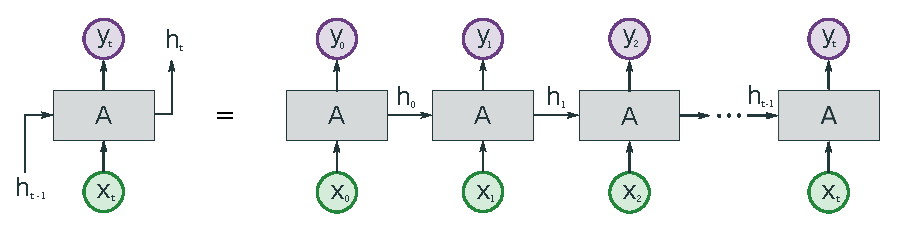
\includegraphics[width=0.8\textwidth]{images/Illustrationen/RNN}
    		\caption{\glqq Ausgerollte\grqq \ Darstellung eines RNN Neurons (inspiriert von \cite{OLAH2015})}
    		\label{fig:RNN}
    	\end{figure}
	    
    Da ein einzelnes Neuron noch keine komplexen Aufgaben lösen kann, ist der Aufbau in Netzen entscheidend.
    Die Neuronen sind in sogenannten \textit{Layers} (z dt. Ebenen) angeordnet (siehe Abbildung \ref{fig:NeuralNet}).
    Es gibt eine \textit{Input-Layer}, quasi beliebig viele \textit{Hidden-Layers} und eine \textit{Output-Layer}.
    Die einzelnen Knoten sind jeweils mit der nachfolgenden Layer verbunden.
    Ist der Ausgang eines Knotens auf einer Layer mit einer vorherigen oder derselben Layer verbunden, spricht man von einem \textit{Feedback} oder \textit{Recurrent Neural Network} (RNN) (siehe Abbildung \ref{fig:RNN}), sonst von einem \textit{Feedforward Neural Network} (FNN). 
    Mit Knoten, die eine extra Verbindung zu sich selbst haben, können frühere Eingaben Einfluss auf die Behandlung der nächsten Eingabe haben.
    Der einzelne Knoten merkt sich seine Ausgabe, welche im nächsten Zeitschritt als weiteres Eingabesignal dient.
    Dadurch wird es ermöglicht auch zeitlich abhängige Sequenzen zu erlernen, da die Behandlung eben auch vorherige Geschehnisse mit einbezieht.
    Lernt ein FNN zum Beispiel die Eingabe (A,B,A,B,A,B,A,\dots), besteht eine 50\% Chance, dass die nächste Ausgabe ein B ist, sofern die letzte nicht bekannt ist.
    Weiß man, dass die letzte Ausgabe ein B war, können wir davon ausgehen, dass eigentlich ein A folgen sollte.
    Die Feedback Struktur RNNs ermöglicht also einen ersten Ansatz, um zeitlich abhängige Muster zu erkennen.
    
    	\begin{figure}[ht]
    		\centering
    		\includegraphics[width=0.8\textwidth]{images/Illustrationen/LSTM}
    		\caption{Schematische Darstellung eines Knotens in einem LSTM NN, mit Input, Output und Forget Gate (inspiriert von \cite{OLAH2015}).}
    		\label{fig:LSTM}
    	\end{figure}
   	
    \textit{Long Short-Term Memory} (LSTM) ist eine Erweiterung der RNNs.
    Hauptziel der LSTMs ist es, das Lernen der zeitlich abhängigen Muster zu verbessern.
    Auch RNNs haben dieses Ziel, doch mit diesen Netzwerken kann schon ein Abstand von 10 diskreten Zeitschritten zwischen den abhängigen Ereignissen nicht überbrückt werden \cite{HOCHREITER1991}. 
    So kann ein RNN zum Beispiel im Satz \glqq Die Wolken am \textit{Himmel}\grqq \ das Wort \textit{Himmel} vorhersagen, doch bei der Satzfolge \glqq Die Person kommt aus Frankreich. ... . Die Person spricht \textit{französisch}.\grqq \ wird es Schwierigkeiten haben.
        %TODO erweitern:
        %doch die größte Schwierigkeit dieser Netze ist das Training. Dabei kommt es häufig vor, dass durch die Back Propagation die berechneten Gradienten entweder verschwindend klein, oder sehr groß werden. Das Bedeutet, dass  Entstehen kann das, 
    Dies soll die LSTM Zelle erweitern und zudem durch verbesserte Fehlerkorrektur für bessere Lernergebnisse sorgen.
    Umgesetzt wird diese Anforderung, indem an jedem Knoten eine \textit{Memory Cell} (Gedächtniszelle) angebracht wird.
    Sie ist mit sich selbst verbunden und gibt den Zellstatus an.
    Mit Hilfe dieser Information soll eine Abhängigkeit auch über einen längeren Zeitraum gefunden werden.
    Der Zellstatus $C_{t-1}$ zum Zeitpunkt $t-1$ hat dann im nächsten Zeitschritt $t$ einen Einfluss auf die Zelle $C_{t}$ und somit auch auf die Ausgabe $y_t$.
    Die Weitergabe des Status wird in Abbildung \ref{fig:LSTM_Status} dargestellt.

    	\begin{figure}[ht]
    		\centering
    		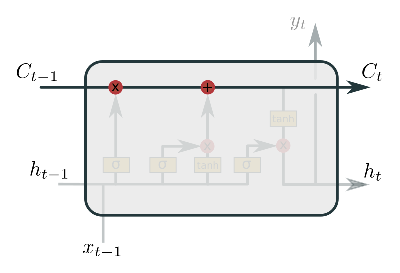
\includegraphics[width=0.5\textwidth]{images/Illustrationen/LSTM_MC}
    		\caption{Weitergabe des Zellstatus innerhalb eines Knotens (inspiriert von \cite{OLAH2015}).}
    		\label{fig:LSTM_Status}
    	\end{figure}
    	
    Einfluss auf den Zellstatus haben zwei verschiedene \textit{Gates} (zu dt. Gatter/Tore).
    Im ersten Schritt wird entschieden, welche Information aus dem vorherigen Zeitschritt keinen Einfluss mehr auf den Zellstatus haben sollen.
    Dies wird mit dem \textit{Forget Gate} umgesetzt und ist in Abbildung \ref{fig:LSTM_Forget} zu sehen.
    Informationen aus dem Speicher, die keinen Einfluss mehr haben sollen, können so entfernt werden.
    In dem Sprachbeispiel könnte das Genus (\textit{grammatikalisches Geschlecht}) gespeichert werden, um so eine grammatikalisch korrekte Vorhersage zu machen.
    Kommt nun allerdings ein neues Pronomen, sollte das bisher gespeicherte Genus keinen Einfluss mehr haben.
    	\begin{figure}[ht]
    		\centering
    		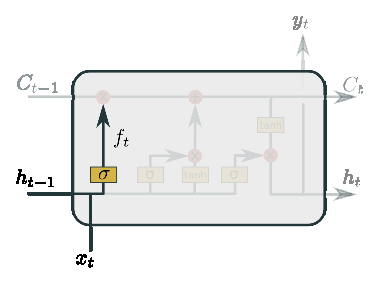
\includegraphics[width=0.5\textwidth]{images/Illustrationen/LSTM_FG}
    		\caption{Einfluss des Forget Gates auf den Zellstatus (inspiriert von \cite{OLAH2015}).}
    		\label{fig:LSTM_Forget}
    	\end{figure}
    	
    Das \textit{Input Gate} soll im nächsten Schritt angeben, welche neuen Informationen in den Zellstatus $C_t$ aufgenommen werden.
    Dies erfolgt in zwei Schritten, zunächst wird mit $i_t$ ermittelt, welche Information geupdated werden soll.
    Im Vektor $\tilde{C}$ ist der eigentliche Werte (wie z.B. das Genus) enthalten, welcher den zuvor vergessenen Wert ersetzen soll (vgl. Abbildung \ref{fig:LSTM_Input}) . 
    	\begin{figure}[ht]
    		\centering
    		\includegraphics[width=0.5\textwidth]{images/Illustrationen/LSTM_IG2}
    		\caption{Einfluss des Input Gates auf den Zellstatus (inspiriert von \cite{OLAH2015}).}
    		\label{fig:LSTM_Input}
    	\end{figure}
    
    Wie der Zellstatus $C_t$ nun die Ausgabe beeinflusst, wird über das \textit{Output Gate} geregelt (siehe Abbildung \ref{fig:LSTM_Output}).
    Dies soll in unserem Sprachbeispiel entscheiden, ob die Information des Genus für die Vorhersage des nächsten Wortes eine Rolle spielt. \cite{GERS2000} \cite{OLAH2015}
    	\begin{figure}[ht]
    		\centering
    		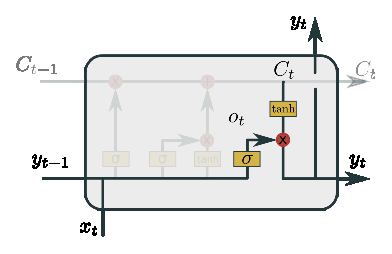
\includegraphics[width=0.5\textwidth]{images/Illustrationen/LSTM_OG}
    		\caption{Das Output Gate regelt den Einfluss des Zellstatus auf die Ausgabe des Neurons (inspiriert von \cite{OLAH2015}).}
    		\label{fig:LSTM_Output}
    	\end{figure}
    
    Die verschiedenen Gates können so als ein weiteres kleines NN in jedem Knoten der LSTM Netze betrachtet werden, welche einen zeitlichen Zusammenhang besser erkennen sollen.
    
